\section{Methodology}
\subsection{Cosmological Parameters}
We considered the parameters of the $\Lambda$CDM model introduced in the Markov chains by the \textit{Planck Collaboration 2018} \cite{planck2018}, namely the reduced density contrast of cold dark matter $\omega_c$ and baryons $\omega_b$, the angular scale of the sound horizon at recombination $100\theta_{MC}$, the amplitude of the primordial spectrum $A_s$, the spectral index $n_s$, and the optical depth to reionization $\tau$. Initially, only the first five cosmological parameters were used, leaving out the optical depth $\tau$. This was due to its well-known temperature degeneracy with the parameter $A_s$.  

\subsection{Simulations}
Since a large number of power spectra need to be simulated by varying the cosmological parameters, it is necessary to adopt a probability distribution from which to initially draw these parameters, known as the \textit{prior}. In this project, a flat prior (uniform distribution) was used within a range of $\pm 10$ sigmas around the fiducial values reported by the \textit{Planck Collaboration 2018} \cite{planck2018}.  

Between 25,000 and 100,000 random samples were drawn from the prior, and for each cosmology a power spectrum of each type ($C_{\ell}^{TT}$, $C_{\ell}^{EE}$, $C_{\ell}^{BB}$, $C_{\ell}^{TE}$) was simulated in the multipole range $0 \leq \ell \leq 2500$. The simulations included only scalar modes (\textit{tensor-to-scalar ratio} \(r = 0\)) and accounted for lensing effects. These simulations were carried out using the \texttt{CAMB} framework in Python \cite{CAMB}. Figure \ref{fig:example_sim} shows three examples for each simulated power spectrum.  

\begin{figure}
    \centering
    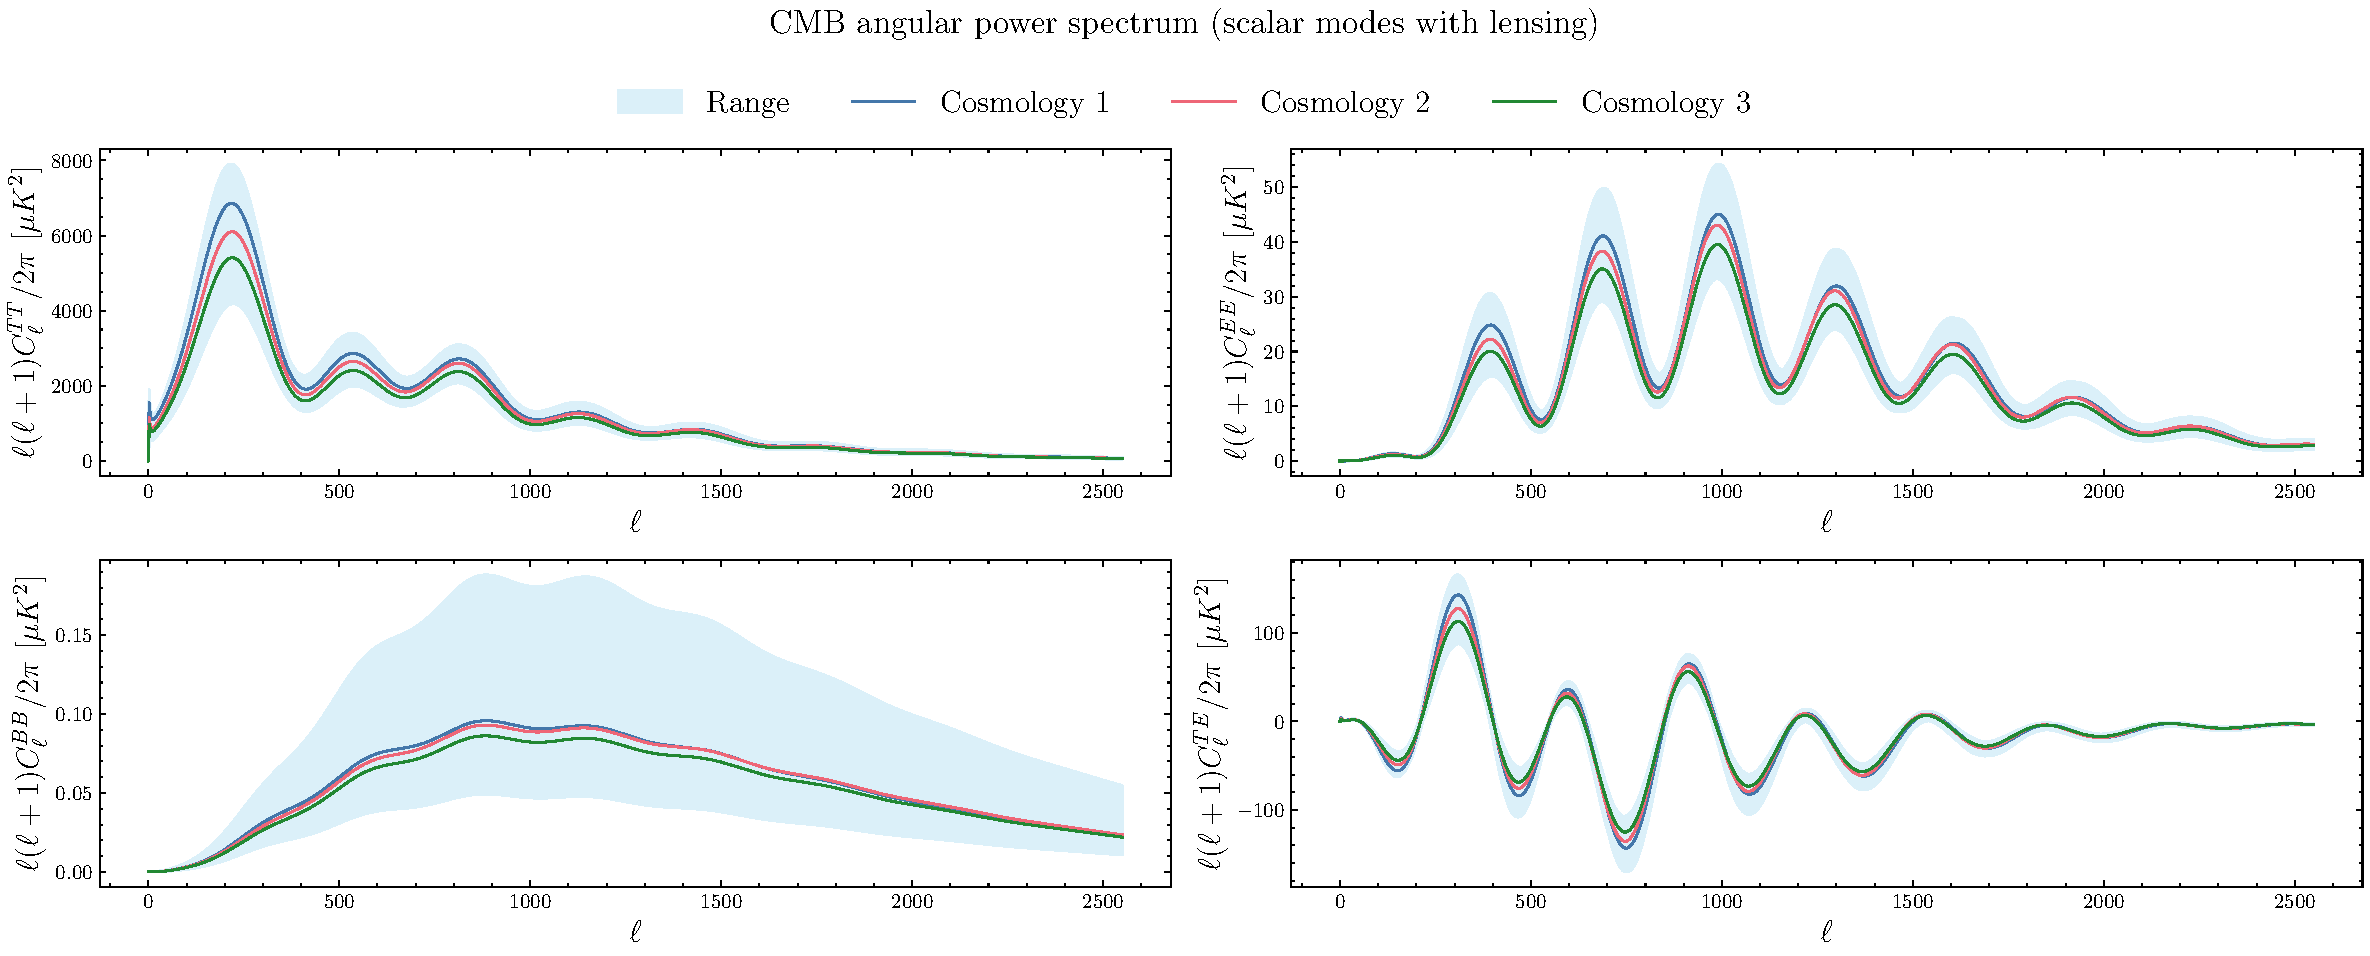
\includegraphics[scale=0.225]{img/cmb_aps_subplot_0.pdf}
    \caption{Example of three simulations of the power spectra $C_{\ell}^{TT}$, $C_{\ell}^{EE}$, $C_{\ell}^{BB}$, $C_{\ell}^{TE}$, respectively. Each simulation was generated from a random sample of the prior.}
    \label{fig:example_sim}
\end{figure}

\subsection{Inference Models}
To estimate the posterior distribution of the cosmological parameters, different inference models were used. In particular, \textit{Sequential Neural Posterior Estimation} \cite{SNPE_C} (SNPE) and \textit{Neural Posterior Score Estimation} (NPSE) \cite{NPSE_1} \cite{NPSE_2} were employed, implemented in the \textit{SBI} Python framework \cite{SBI}. Both NPSE and SNPE are Bayesian inference methods for simulation-based models, but they differ in their representation of the posterior and their training mechanisms. NPSE uses conditional diffusion models and \textit{score matching} to estimate density gradients, thereby avoiding the use of normalizable models \cite{NPSE_1}, while SNPE-C employs \textit{normalizing flows} to directly model the posterior and requires importance-weighting corrections \cite{SNPE_C}. In the specific case of this project, NPSE showed better adaptation to the data, producing wider but less biased posteriors than SNPE, as shown in Figure \ref{fig:model_comparison}.  

\begin{figure}
    \centering
    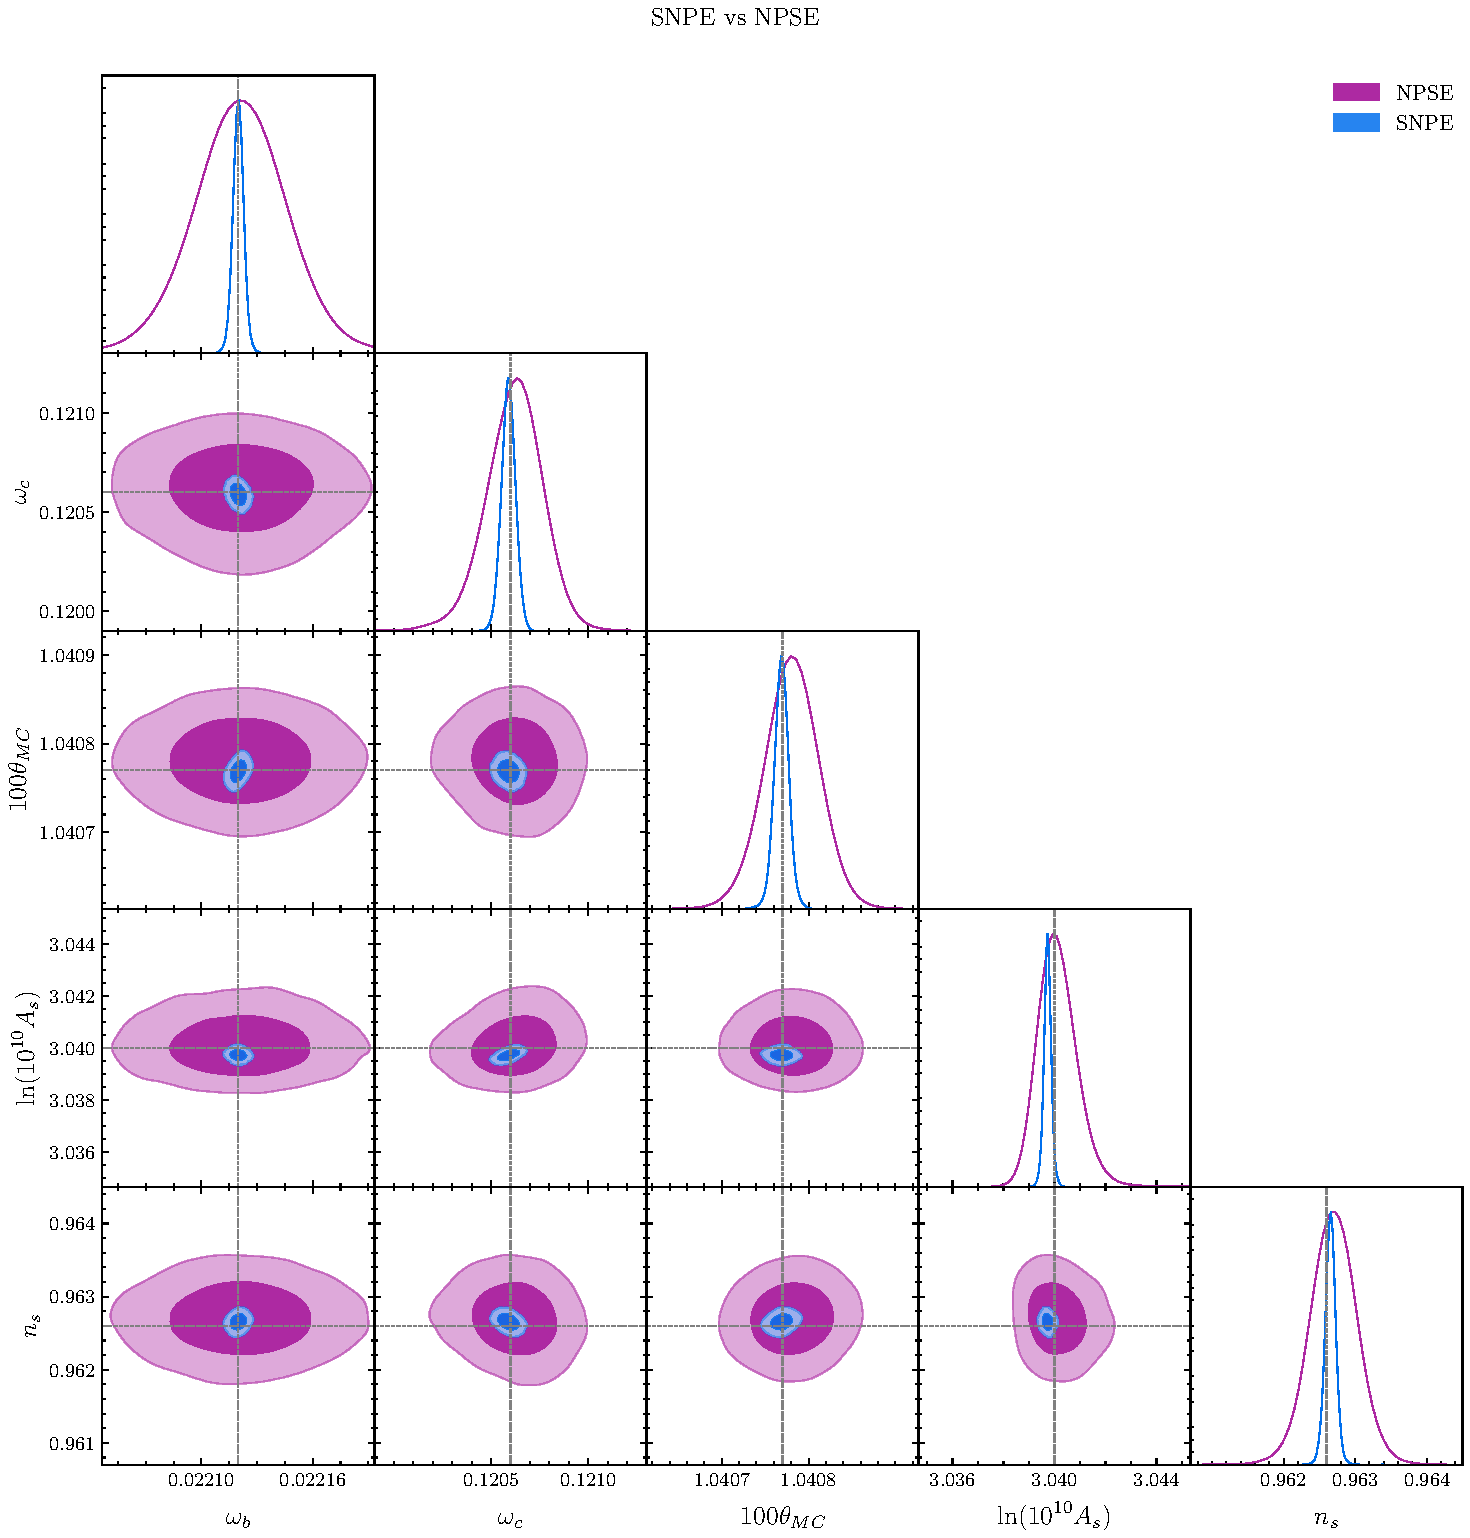
\includegraphics[scale=0.35]{img/inference_model_comparison.pdf}
    \caption{PPC diagnostic of the results obtained with the inference models SNPE and NPSE. Both models were trained with the same 100,000 simulations of the $C_{\ell}^{TT}$ power spectrum. The dashed line indicates the true value of the parameters. The NPSE model yields wider but less biased distributions compared to SNPE.}
    \label{fig:model_comparison}
\end{figure}

\subsection{Posterior Predictive Check (PPC)}
The result of training the selected inference model is known as a density estimator, which is capable of generating random samples from the trained posterior distribution given an observation. To analyze and evaluate the quality of the model, the \textit{Posterior Predictive Check} (PPC) \cite{SBI} method was used. This consists of selecting a true value for the cosmological parameters and simulating an observed power spectrum, and then sampling the previously trained posterior distribution from this observation. In this way, the posterior distribution obtained by the inference model can be compared with the true parameter value, typically represented by a dashed line, as shown in Figure \ref{fig:model_comparison}.



